\documentclass{article}

\usepackage{indentfirst}

\usepackage{amsmath}
\usepackage{amssymb}
\usepackage{geometry}
\usepackage[utf8]{inputenc}
\usepackage{graphicx}


\graphicspath{ {images/} }
\setlength{\arrayrulewidth}{1mm}
\setlength{\tabcolsep}{18pt}
\renewcommand{\arraystretch}{1.5}

\geometry{left = 2.0cm,	right = 2.0cm,	top = 2.0cm, bottom = 2.0cm}

\title{Portfolio of MSSP Projects}
\author{Zichun Liu}

\begin{document}
	\maketitle
	\tableofcontents
	.\\
	.\\
	.\\
	.\\
	.\\
	.\\
	\section{Overview}
	The purpose of this portfolio is to show the work of MSSP students on collaborative consulting projects. Throughout two semesters, students in MSSP formed the consulting groups and solved problems from the clients who were either within BU at different departments or outside of BU. We helped them with their research projects and provided statistical solutions by all kinds of ways. This portfolio consists of separate sections which summarize the background, data, modeling and findings of every project. The links to the codes on GitHub for most of the projects are in the reference section at the end of the portfolio. Due to some restrictions, some data and codes of the projects remain confidential. In this portfolio, I archived eight main projects:
	\begin{itemize}
		\item Ant anatomy and behavior research
		\item Catalog study on women emancipation
		\item Salmon habitation preference study
		\item Visualization for Boston University Women Soccer Team
		\item Measuring the impact of geriatric care among Medicare beneficiaries
		\item R package: Single cell toolkit
		\item Random Contamination and Select Response Styles affecting measures of fit and reliability in factor analysis
		\item R package: celda - Cellular Latent Dirichlet Allocation(ongoing)
		\item Recommender system on Consumer Unit dataset(ongoing)		
	\end{itemize}

	\section{Measuring the impact of geriatric care among Medicare beneficiaries}
	This is a collaborative project conducted by the MSSP consulting team and Trinity Partners, LLC. The outcome was accepted by 22nd ISPOR annual meeting as a poster presentation. 
	\subsection{Introduction \& Background} 
	In 2015, there are almost 50 million people over 65 and 70 percent of them have two or more chronic conditions, which contributes to non-stopping, continuing costs of medicine and other medical services. In the previous studies geriatricians, doctors who meet the unique healthcare need of older adults, have been shown to have an influence on elderly patients, especially those with severe chronic diseases. 
	
	To form a better view of the impact of geriatrician on the aging population, we modeled the Medicare claim data between January 2010 and January 2015 to infer the effect of geriatric care on \textbf{longevity, cost, and the use of medical resources}. This paper measures the impact of geriatric care on patient outcomes
	
	\subsection{Data Format}
	The study cohorts were created from claims spanning 2010-2014, representing a random 5\% sample of Medicare FFS beneficiaries that were aged 65+ in 2010. Patients with at least one geriatric care claim between (but not before) 2011-2014 were propensity score matched to those without any geriatric care claims from 2010-2014.
	
	For the purpose of studying the impact of geriatric care on patients, we converted the claim-based data to patient-based data. The number of claims in 2010 and CCI are calculated from the information between 2010-01-01 and 2010-12-31. Other variables are calculated or extracted from information between 2011-01-01 and 2014-12-31. 
	
	2 pair of sample datasets have been used in the analysis, being one for survival analysis and the other for cost and resource analysis.
	
	\subsection{Modeling \& Analysis}
	\subsubsection{Methods}
	To draw casual relationship from the Medicare data, a matched cohort analysis, \textbf{propensity score matching}, was performed, we used comparing patient outcomes among those with and without geriatrician care. \textbf{Survival rates, healthcare resource utilization (HCRU) and costs} were compared between matched cohorts.
	
	\paragraph{Propensity score}is the probability of being assigned treatment conditional on observed covariates, which we denote as $P(T=1|X)$. Here $X$ indicates a matrix of all pre-treatment covariates, $T$ indicates binary treatment corresponding to geriatric care. $T$ is 1 when there is geriatric care and $T$ is 0 when there is not. 
	
	Propensity score matching entails forming matched sets of subjects in case and control groups, who share a similar value of the propensity score. Subjects in case and control groups that are paired are close to each other, which is done by using nearest neighbor matching method.
	
	\begin{figure}[h]
		\centering
		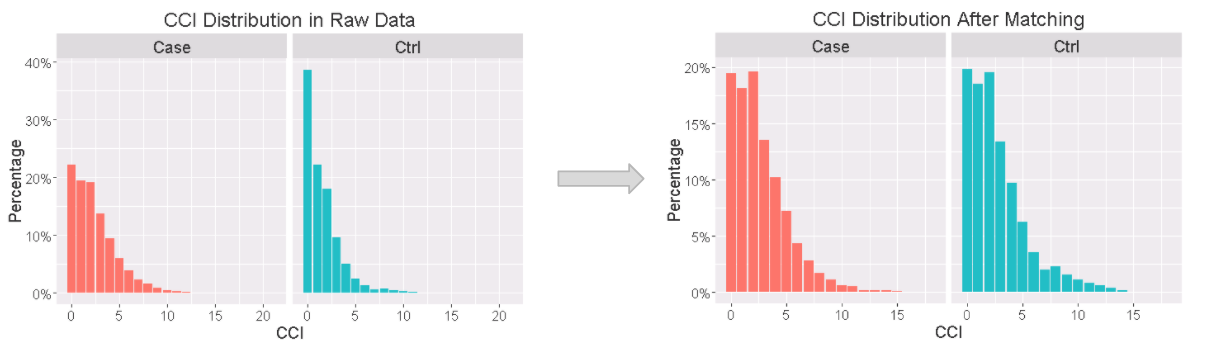
\includegraphics[width=1\textwidth]{TrinityPSM}
		\caption{Propensity Score Matching}
	\end{figure}


	\paragraph{Survival Analysis} were performed to investigate the impact of geriatric care on longevity. The Kaplan-Meier estimate is a famous nonparametric maximum likelihood estimate of the survival function. The estimate is a step-wise empirical function which can be written as:
	\begin{align*}
	\hat{s}(t) &= 1, if \indent t < t_i\\
	\hat{s}(t) &= \prod_{t_i\le t}[1 - \frac{d_i}{Y_i}], if \indent t \ge t_i
	\end{align*} 
	
	Where we have order the event times as a sequence of ascending, e.g. $0 < t_1 < t_2 < ... < t_D$ . di is how many of individuals with an observed event at time $t_i$ and $Y_i$ is the number of individuals who are at risk at time $t_i$.
	
	And to make an accurate and solid comparison between the case and control groups in terms of the survival analysis, we constructed a Weibull regression model. The survival function for the Weibull distribution is:
	$$S_T(t) = e^{-\lambda t^P} $$
	
	Where $\lambda$ is reparameterized in terms of predictor variables and regression parameters, and $p$ is the shape parameter which is held fixed for a parametric model.
	
	\begin{figure}[h]
		\centering
		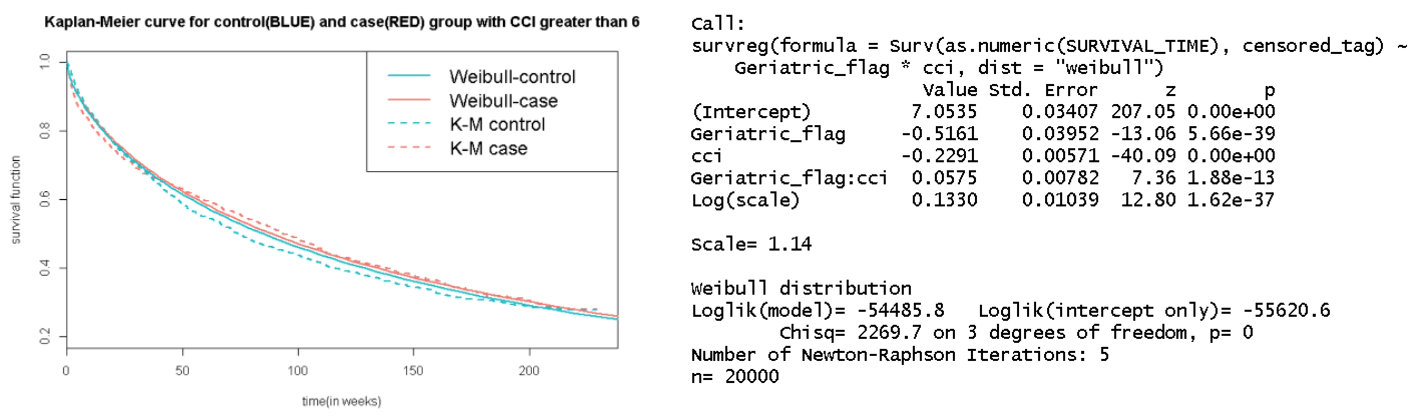
\includegraphics[width=1\textwidth]{TrinitySurvival}
		\caption{Survival Analysis}
	\end{figure}
	
	\paragraph{Cost analysis}used T-test after propensity score matching to compare the cost between case and control groups. 
	\paragraph{Resource Utilization analysis} used Linear Regression Models after propensity score matching to compare the medical resources usage. The response variables are: Log-transformed claim numbers and log-transformed length of stay in hospital; The independent variable is whether there is geriatric treatment.
	
	\subsubsection{Results}
	118,382 patients receiving geriatric care were identified, along with a random sample of 535,526 patients not receiving geriatric care. Samples of the cohorts were taken and propensity score matching was performed to create 10,000 matched pairs. Kaplan-Meier plots comparing the two matched cohorts indicated that, overall, the geriatric care group had shorter survival times than their counterparts. Among sicker patients, however, the analysis suggested that survival times were relatively longer in the geriatric care group. In terms of HCRU, patients receiving geriatric care were, on average, likely to have more inpatient, outpatient and physician office claims (62\%, 18\% and 49\% more, respectively). Mean monthly costs were comparable in the two matched cohorts (p=0.53).
	
	
	\subsection{Conclusions}
	Geriatric care has the potential to improve the longevity of those afflicted by multiple chronic conditions. Geriatricians’ focus on coordination of care increases the amount of healthcare resource utilization but costs are on par with patients not receiving geriatric care, possibly the result of support that is more efficient and preventative in nature. While only a small proportion of elderly patients receive geriatric care, this study suggests that more patients and the healthcare system at large could benefit from promoting the involvement of and increasing access to geriatricians.
	\subsection{Discussion}
	\subsubsection{Quality of Life}
	There’s another aspect of life that’s not covered in our data – quality. How much pain or distressing physical symptoms do they experience on a daily basis? Are they depressed, anxious or do they sleep well at night? Most importantly, their functional status, are they highly dependent or able to manage ordinary, mundane daily activities? It’s also of great interest and importance to investigate whether geriatricians can make a difference for elderly in this aspect, for life has much more dimensions than just time and money. Therefore, for future analysis, another angle is to assess the quality of life of those elderly patients treated by geriatricians.
	\subsubsection{Side effect of overuse of geriatric care on cost}	
	For all case sample we have had resampled from the raw data, cost first decrease to the bottom until the number of months having geriatric care is around 25, and then cost increase after that. This also indicates that geriatric care won’t increase cost for patients or even decrease cost at first, but overuse of geriatric care can have side effects on cost.
	\subsection{Appendix}

	\section{Ant anatomy and behavior research}
	\subsection{Introduction \& Background}
	In this project, our client Darcy Gordon from Department of Biology is interested in the relationship between ant brain anatomy and motor information. Our team mainly focused on helping our client analyze the result of her experiment. The experiment focused on 3 types of ants(3 morphological groups) from 3 colonies and tested their ability to detect chemical trails with different concentrations. 

	Based on our conversations, client is interested in:
	\begin{enumerate}
		\item Effect of the subcaste and the trail concentration on the success rate of detection for each ants. This can be broken down into:
		\begin{itemize}
			\item Does concentration increase the detection rate.
			\item Is there a difference in the detection rate between the subcaste.
			\item Is the effect of concentration differeren for different subcaste.
		\end{itemize}
		\item Prediction for different subcaste and a trail concentration with the prediction interval.
	\end{enumerate}
	
	\subsection{Data Format}
	Because each individual ant was tested at each of the 3 chemical trails. The whole data set has 3*(17+18+17) = 156 observations. 
	
	There are two kinds of outcomes, the first one is binary(detection or not,1 or 0), the second one is the proportion of detected trail crosses (on a scale of 0-1). It gives us information about how well they followed a trail not just if they are able to detect it. 
	
	However, the turns and crosses have more information than the proportions. The detection data could be treated that it is from the proportions (0 proportions indicate 0 detection while not 0 proportions indicate 1 detection).
	
	

	\subsection{Modeling \& Analysis}
	\subsubsection{Methods}
	After the discussion with our client, we agreed to work on the following two models: \\
	
	\noindent\textbf{Model 1: Binomial Model with turns and crosses information as responses}  

	\begin{align*}
	y_i &\sim Binomial(n_i,p_i)\\
	p_i &= logit^{-1}(\beta_0 + \beta_sx_{is} + \beta_cx_{ic} + \beta_{sc}x_{is}:x_{ic} + \alpha_{j[i]})\\
	\alpha_j &\sim N(0, \sigma^2_a),j=1,...,J
	\end{align*}
	
	Where $i$ indexes each trial, and $j$ indexes each ant. In this model we assume turns and crosses are successes and failures of sequence of independent trials, which is not necessarily true. However by accounting for $n_i = trun_i + cross_i$ we are in a way taking into account the indivisual activity level. We assume the turns and crosses are independent.  \\
	
	\noindent\textbf{Model 2: Logistic Regression with binary outcomes as responses}  
	
	\begin{align*}
	y_i &\sim Bernoulli(p_i)\\
	p_i &= logit^{-1}(\beta_0 + \beta_sx_{is} + \beta_cx_{ic} + \beta_{sc}x_{is}:x_{ic} + \alpha_{j[i]})\\
	\alpha_j &\sim N(0, \sigma^2_a),j=1,...,J
	\end{align*}  
	
	Where $i$ indexes each trial, and $j$ indexes each ant. In this model we collapsed the crosses and turns information into binary outcomes, that is, if the number of turns is not zero, then there is a success (outcome 1) for this single trial which includes multiple turns and crosses. We assume these macro trials are independent.

	\subsubsection{Model 1 Results}
	\paragraph{linear separation problem}
	At first we enroll the interaction term in the logistic mixed effect model. We found something strange happens: the standard error of $subcasteminor:concentrationlow$ is extremely large. It is called the linear separation problem. This phenomenon happens due to the sudden change in response when we change the value of discrete predictors. 
	
	\paragraph{Remedy}One necessary condition of linear separation is that all the predictors should be discrete, so one simple remedy method is to use continuous concentrations: 0.0003, 0.001, 0.003. Because we are considering interaction term, the scales of predictors should be almost the same. I multiplied each concentration by 1000.
		
	\begin{figure}[h]
		\centering
		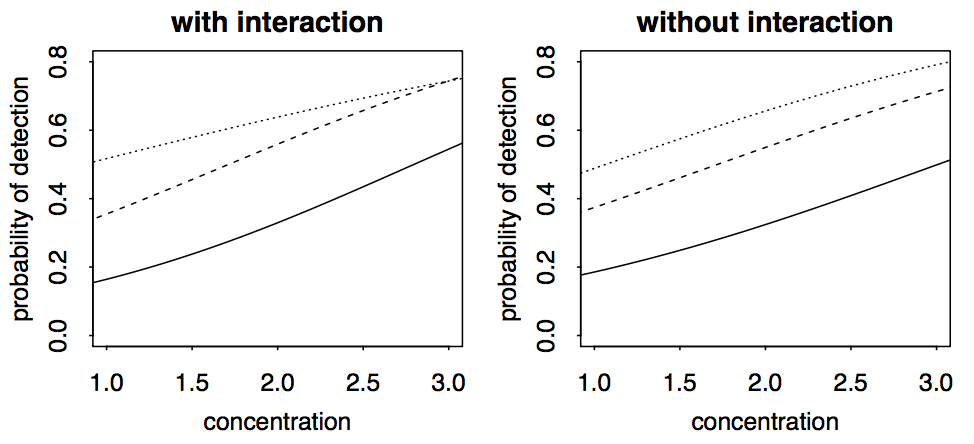
\includegraphics[width=0.8\textwidth]{AntModel1plot}
		\caption{Model Fit}
	\end{figure}
	
	\paragraph{Prediction}
	If we don’t specify the ant ID in prediction, we need to add variance from random effect and get larger prediction intervals. If we use ant ID in prediction, we will get small prediction intervals. The corresponding results are generated through 'predictInterval' function in R.
	\subsubsection{Model 2 Results}
	\paragraph{Linear separation problem and remedy}
	Using predictor “concentration” with 3 levels low, medium, high, we came across the linear separation again. And as what we have done in the last section, use numeric concentration and again scale them (times 1000) and refit the model.
	
	The interaction terms are not significant, but the signs before the coefficients of the interactions are the same as those in Section 4.2. Keeping the interaction term will not hurt the predictions. The plots below also showed that there is some difference between the left and right plot, although not significant.	
	
	\begin{figure}[h]
		\centering
		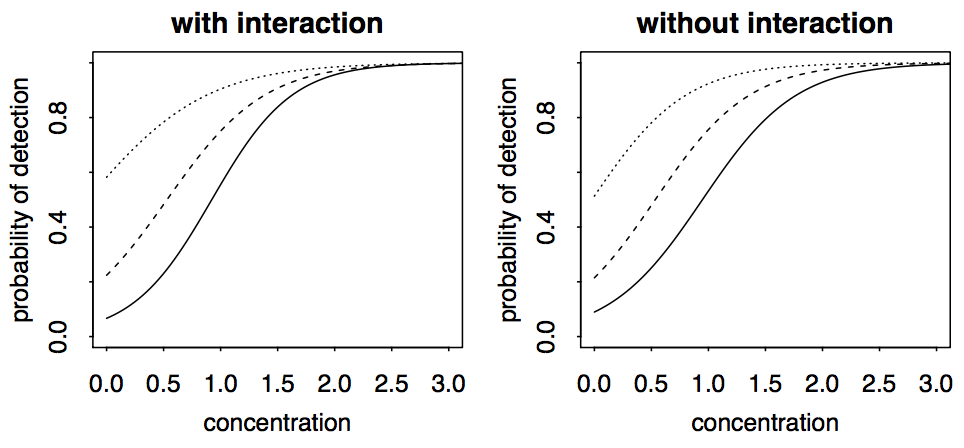
\includegraphics[width=0.8\textwidth]{AntModel2plot}
		\caption{Model Fit}
	\end{figure}
	
	\paragraph{Prediction}
	We can get similar prediction interval for each combination of subcaste and concentration level without ant ID, via the same simulation method. The prediction intervals are also generated through 'predictInterval' function in R.
	
	\subsection{Conclusion}
	From both models, we can see obviously that the increase in concentration will increase the detection rate. And different ants have a distinction in detecting chemical trails: Supersoldiers have the highest detection rate and Minors have the lowest detection rate. What's more, we may tell that the effect of concentration is different for different subcaste from the interaction term in our model.
	
	\subsection{Discussion}
	\subsubsection{Limitations of our analysis}
	There are some limitations of our analysis, because of these two assumptions we made: 
	\begin{enumerate}
		\item We are assuming the turns are independent from one another, which we have known they are not true.
		\item We are assuming homogeneity across the colonies, because we don’t include colony effect in our analysis. See Section 2.5.2.
	\end{enumerate} 
	
	\subsubsection{More about random effect: the colony effect}
	We tried putting the colony effect in the model but we encountered numerical issues again and had some problems in convergence. Thus we were unable to include the colony effect by now. If you want to add colony effect urgently, we are happy to work on applying the regularization methods mentioned below to address the numerical issues and include colony effect into analysis. In other case, we’d like to include ant ID as random effect only as what we did in Section 2.1-2.4.
	
	\subsubsection{Future analysis: fully addressing the numerical issues}
	To fully address the numerical issues including linear separation, we would probably need to use some regularization methods in Bayesian framework. The Bayesian regularization methods won’t provide p-values which is required in many fields. We will be happy to make suggestions if our client's field don’t have a strict rule about providing p-values.
	
	\section{Catalog study on women emancipation}
	\subsection{Introduction \& Background}
	In this project, our client Ashley Tartarilla from Department of Psychological and Brain Sciences is interested in the relationship between levels of gendered nonverbal behavior to levels of women's emancipation for each country represented. To help our client approach to their research goals, our team mainly focused on analyzing the data.
	
	Our client have qualitatively coding images from toy catalogs from different countries worldwide for gendered nonverbal behavior. Based on our conversation, client is interested in: 
	\begin{enumerate}
		\item Recategorized 38 measurements into 6 variables
		\item Compute a table of proportions, for each gender, for each country, for each composite variable
		\item Perform T-test and permutation test between genders for each of the 6 coding variables and visualised them
		\item Convert the test scores from T-test and permutation test into z-scores by the inverse probability transformation and do some visualization
	\end{enumerate}

	\subsection{Data Format}
	To be added
	
	\subsection{Modeling \& Outcome}
	\subsubsection{The two-sample t-statistics and converted z scores}
	According our clients’ advice, we created composite scores by grouping similar variables together. Initially we have 38 variables for each gender, after grouping we have 3 composite variables for each gender, 6 in total: Feminine emotional expression, Masculine emotional expression, Feminine nonverbal behavior, Masculine nonverbal behavior, Feminine objects in picture and Masculine objects in picture. 
	\subsubsection{The two-sample t-statistics and converted z scores}
	We computed the two-sample t-statistics between genders for each country and each composite variable.Since we have 20 countries and 6 composite variables, we have conducted 120 t tests totally and a t-statistic matrix with 20 columns(countries) and 6 rows(composite variables) was computed. These t tests have different degrees of freedom due to different sample size, so we converted the all the 120 t statistics into standard normal distribution scale by inverse probability transformation, for more convenient illustration.
	\subsubsection{The Permutation test p values and converted z scores}
	For formal testing, permutation tests are more reliable for our experiment compared with t-tests; as t-test requires normality of samples. So we conducted permutation tests between genders for each country and each composite variable, following the same logic as the t tests described above. Again, since we have 20 countries and 6 composite variables, we have conducted 120 permutation tests totally, and constructed a matrix of permutation tests p values, with 20 columns(countries) and 6 rows(composite variables). P values of permutation tests measures the probability of the 2 vectors being tested coming from the same distribution, and the values range from 0 to 1. We then converted all the 120 p values into standard normal distribution scale(converted z scores), by inverse probability transformation.
	\subsubsection{Data Visualisation and interpretation of heatmaps}
	Even though ‘T tests Z-scores Heatmap’ gives us similar results, we focus on the interpretation of ‘Permutation Z-score Heatmap’; since permutation tests results are more reliable in our experiment. Generally, we can see 3 kinds of colors in the heatmap. The color purple means ‘no significant difference’, color blue means ‘girls are doing this more than boys’, color red means ‘boys are doing this more than girls’.
	
	\begin{figure}[h]
		\centering
		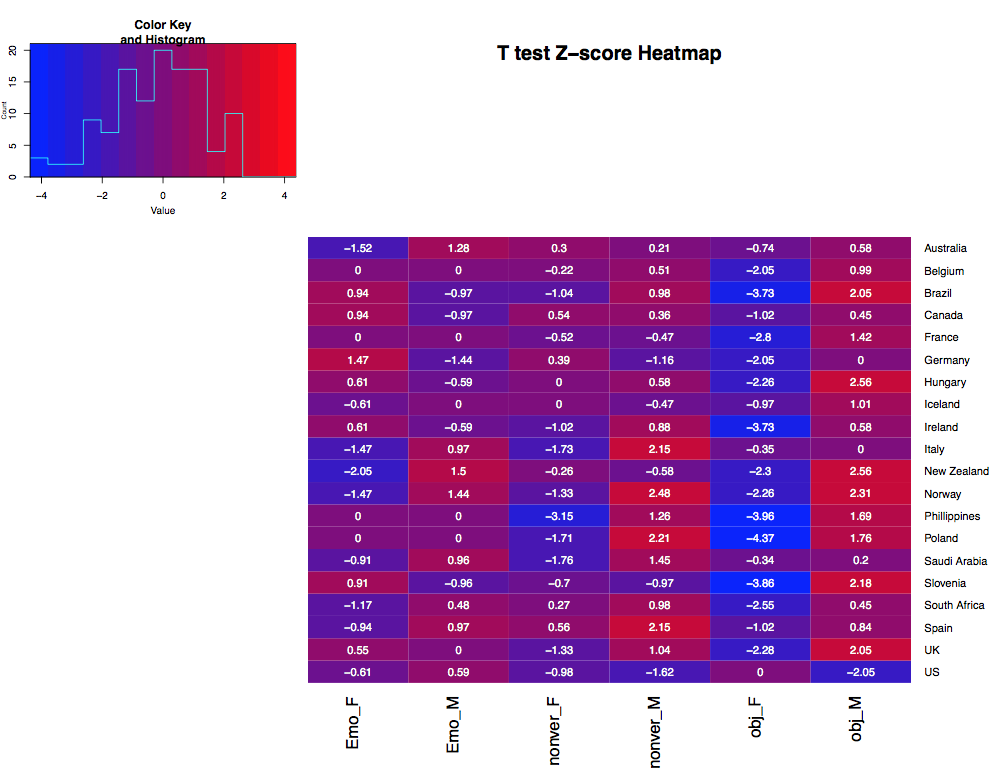
\includegraphics[width=0.8\textwidth]{CatalogHeatmap1}
		\caption{Heatmap T test}
	\end{figure}
	
	\begin{figure}[h]
		\centering
		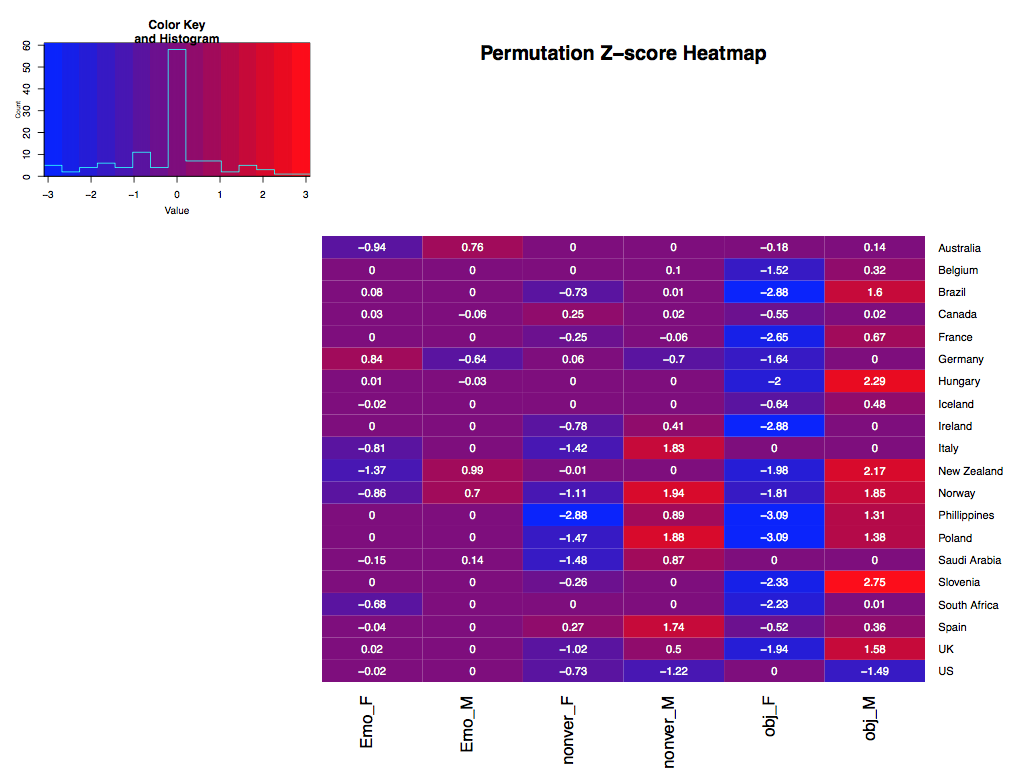
\includegraphics[width=0.8\textwidth]{CatalogHeatmap2}
		\caption{Heatmap permutation test}
	\end{figure}
	
	We have some really interesting findings. Regarding ‘Feminine Emotion Expression’ and ‘Masculine Emotion Expression’, we can see that there is not much difference across the countries. Nonverbal behavior differences between genders are more obvious, while objects in picture differences are significant cross most of the countries.
	\subsubsection{Correlation between permutation\&t tests z-scores and GGI}
	We calculated the correlation between GGI of each country and visualised it. To interpret this plot, differences in feminine nonverbal behaviors, feminine emotion expression and masculine objects are positively correlated with GGI; the difference in feminine nonverbal behaviors has the largest positive correlation with GGI. While differences in feminine objects, masculine nonverbal behaviors and masculine emotion expression are negetively correlated with GGI.
	
	\begin{figure}[h]
		\centering
		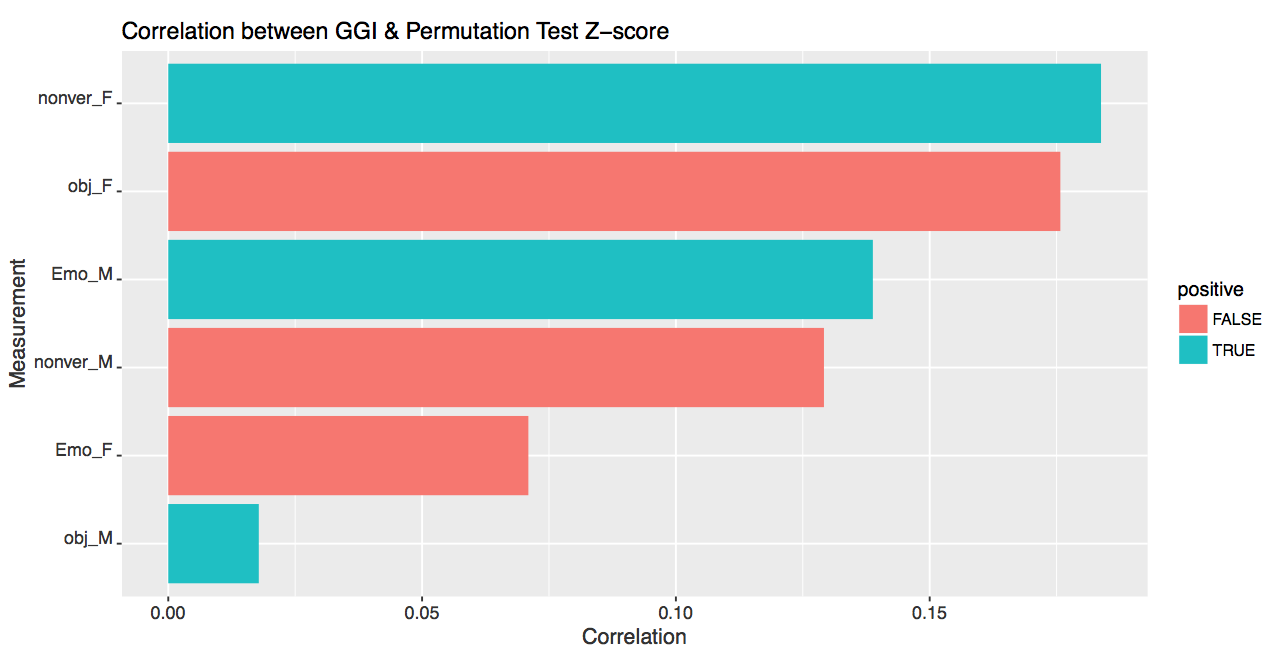
\includegraphics[width=0.6\textwidth]{CatalogCorrelation}
		\caption{Correlation Between GGI and permutation test scores}
	\end{figure}
	
	\subsection{Conclusion}
	In this project, our client mainly want some visualization result to support their theory. And after discussion we have some very practical tasks. Through our work. We can have a better sense of how Women's emancipation in a country can be related to some of nonverbal behaviors of children by compress measurements into composite variables and perform permutation tests.
	
	\section{Salmon habitation preference study}
	\subsection{Introduction \& Background}
	Our client David Minkoff is from BU Marine Program. In his project, Juvenile salmon were placed in a 2-choice maze to determine preference between 2 odors administered into the water column. Laminar flow was established through the maze, ensuring that no mixing of odors occurred from one side to the other. The location of the fish on one or the other side of the maze was observed every 5 seconds for a duration of 2 minutes, after which the sides on which odor was administered was switched. The location of the fish was again observed for an additional 2 minutes (number of data points per fish = 24 time points before odor side-switch + 24 time points after side switch = 48 total data points per fish). Three different odor choice scenarios were tested with n=36 fish for each scenario.
	
	Our client came to with with research question: Do fish prefer the odor to expose when they grow-up over the others? And his expectation is that fish prefer the odor to expose when they grow-up over the others. 
	\subsection{Data Format}
	The data we used was our client's experiment data. In his experiment, there are 3 kinds of odors: A, B and C:
	\begin{itemize}
		\item A: well/brook water with Arginine, for fish from well/brook water accordingly
		\item B: odor given off by other fish
		\item C: control, which is still water
	\end{itemize}
	
	There are two kinds of environments: Brook water and well water. And within each environment, half of the fish are raised with treatment, half are control group.
	
	The experiment are done as follows, the rows show the average proportion of (turn to A)/(Total record)
	
	\begin{tabular}{ |p{2cm}||p{2cm}|p{2cm}|p{2cm}|p{2cm}|  }
		\hline
		\multicolumn{5}{|c|}{Experiments} \\
		\hline
		Tables& Well water treatment &Well water control &Brook water treatment &Brook water control\\
		\hline
		A vs B   & 0.44, N=35   &0.42, N=36&0.56, N=36&0.48, N=36\\
		A vs C 	 & 0.44, N=36  	&0.44, N=36&0.52, N=36&0.50, N=33\\
		\hline
	\end{tabular}\\
	
	When we focus on the table: A vs B and A vs C, the treatment proportions are a little higher, which is a weak evidence supporting the expectation.

	According to the research question and the data format, we choose to use if the fish turned to Arginine as response, which is binary when we decomposing the original data into independent measures. That is, take each measurement as an observation.
	
	Predictors are:
	\begin{itemize}
		\item Hatch in Brook water (True or False)
		\item Hatch in Treatment (True or False)
		\item Arginine on Left (True or False)
		\item the other odor (B or C)
	\end{itemize}

	Note that if don’t use the whole data, some predictors can’t be added in. We will discuss it more in the following sections. 
	
	Random effect: fish ID

	\subsection{Modeling \& Analysis}
	\subsubsection{Exploratory Data Analysis}
	We are interested in how fish (treatment or control) perform in A vs B or C condition, so we make the following plot:
	
	\begin{figure}[h]
		\centering
		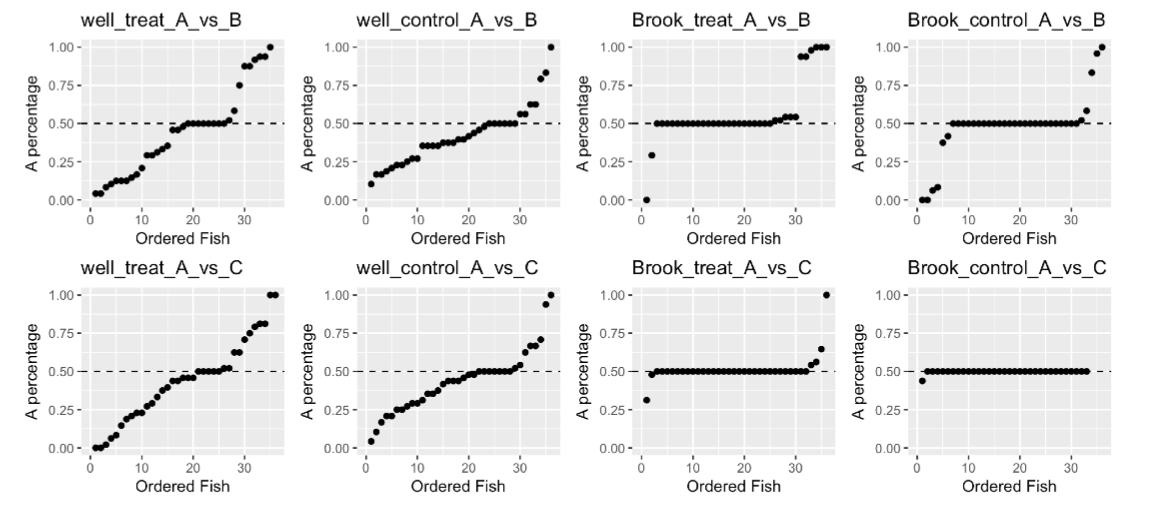
\includegraphics[width=1\textwidth]{EDAsalmon}
		\caption{EDA}
		\label{fig:eda_salmon}
	\end{figure}
	
	Controlling other conditions the same and varying the fish grow-up condition (treatment or control), for example, comparing well treat A vs B and well control A vs B. We will always find the result always tends to support the expectation in Section 5.1, although the evidence still seems weak.
	
	\subsubsection{Modeling}
	Let us not consider the interaction effect in this part. We perform the following modeling:
	\begin{enumerate}
		\item Model 1: combine “Brook Control A vs B”, “Brook Treatment A vs B”, predictors: “Hatch with Treatment”, “Arginine on Left”, random effect: “Fish ID”
		\item Model 2: combine “Brook Control A vs C”, “Brook Treatment A vs C”, predictors: “Hatch with Treatment”, “Arginine on Left”, random effect: “Fish ID”
		\item Model 3: combine all the 4 data sets, predictors:“Hatch with Treatment”, “Arginine on Left”, “the other odor”, random effect: “Fish ID”.
	\end{enumerate}
	.\\
	.\\
	.\\
	.\\
	.\\
	.\\
	.\\
	.\\
	.\\
	.\\
	.\\
	.\\
	.\\
	.\\
	.\\
	\subsubsection{Analysis}
	\paragraph{Model 1}
	We fit the model 1 and the results are as follows:
	\begin{figure}[h]
		\centering
		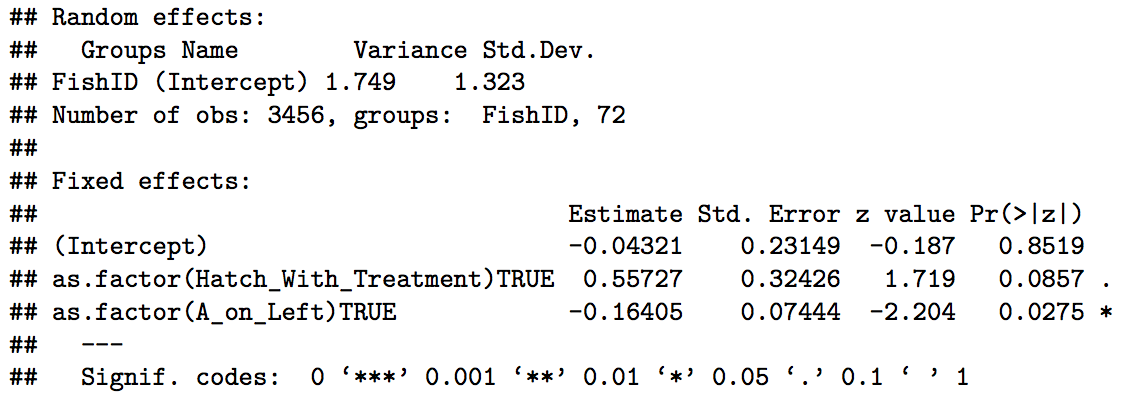
\includegraphics[width=1\textwidth]{Salmonmodel1}
		\caption{Model1}
	\end{figure}
	
	From the p-value and coefficient of Hatch with Treatment, support the expectation, but only nearly significant.
	
	\paragraph{Model 2}
	We fit the model 2 and the results are as follows:
	\begin{figure}[h]
		\centering
		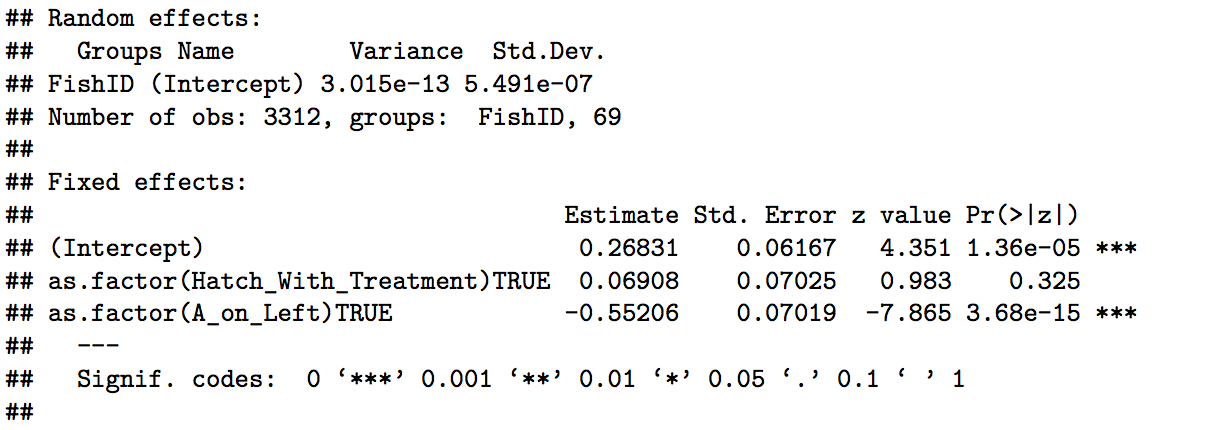
\includegraphics[width=1\textwidth]{Salmonmodel2}
		\caption{Model2}		
	\end{figure}
	
	From the p-value and coefficient of Hatch with Treatment, support the expectation, but not significant.
	.\\
	.\\
	.\\
	.\\
	.\\
	.\\
	.\\
	.\\
	.\\
	.\\

	\paragraph{Model 3}
	Finally we fit the model 2 and the results are as follows:
	
	\begin{figure}[h]
		\centering
		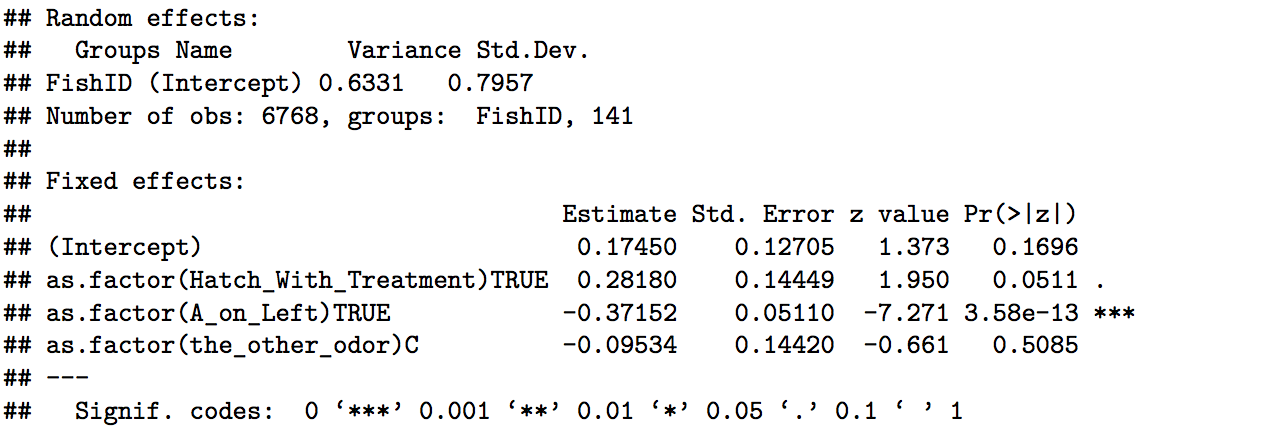
\includegraphics[width=1\textwidth]{Salmonmodel3}
		\caption{Model3}
	\end{figure}
	
	From the p-value and coefficient of Hatch with Treatment, support the expectation, but only nearly significant. It seems that the other odor will not affect the preference of fish, because the p-value of ‘the\_other\_odor’ suggest that this coefficient is not significant.
	
	\subsection{Conclusion}
	We approach to the answer through descriptive statistics, EDA and statistical modeling, and we see the results from Data Description, EDA and Modeling Part in Section 3 agree with each other. That is, fish do prefer the odor to expose when they grow-up over the others. However, that preference impact is very weak that may be concealed behind a strong side-effect, that is, fishes are very likely to turn to right regardless of the environment.


	\section{Visualization for Boston University Women Soccer Team}
	\subsection{Introduction \& Background}
	test
	\subsection{Data Format}
	\subsection{Visualization}
	\subsection{Discussion}	
	
	\section{R package: SingleCellTK(ongoing)}
	asdf
	\subsection{Introduction \& Background}
	sadf
	\subsection{Data Format}
	asdf
	\subsection{Modeling \& Analysis}
	adsf
	\subsection{Conclusion}
	asdf
	\subsection{Discussion}
	asdf

	\section{R package: Celda(ongoing)}
	asdf
	\subsection{Introduction \& Background}
	asdf
	\subsection{Data Format}
	asdf
	\subsection{Modeling \& Analysis}
	asdf
	\subsection{Conclusion}
	asdf
	\subsection{Discussion}
	adsf
	
	\section{Random Contamination and Select Reponse Styles affecting measures of fit and reliability in factor analysis(ongoing)}
	asdf
	\subsection{Introduction \& Background}
	asdf
	\subsection{Data Format}
	asdf
	\subsection{Modeling \& Analysis}
	asdf
	\subsection{Conclusion}
	adsf
	\subsection{Discussion}
	adsf
	
	\section{Recommender system on Consumer Unit dataset(ongoing)}
	adsf
	\subsection{Introduction \& Background}
	asdf
	\subsection{Data Format}
	asdf
	\subsection{Modeling \& Analysis}
	asdf
	\subsection{Conclusion}
	asdf
	\subsection{Discussion}
	asdf
	
	\section{Acknowledgements}
	Projects included in the portfolio received support and guidance from:
	\begin{itemize}
		\item Professor Eric D. Kolaczyk in the Mathematics and Statistics at Boston University.
		\item Professor Masanao Yajima in the Mathematics and Statistics at Boston University.
		\item Professor Gregg A. Harbaugh in the School of Education at Boston University
		\item Teaching fellow Jun Li in the Mathematics and Statistics at Boston University.
	\end{itemize}
	\section{Reference}
	Projects available at https://github.com/lloydliu717/Portfolio

\end{document}